\documentclass[a4paper]{article}

%% Language and font encodings
\usepackage[english]{babel}
\usepackage[utf8x]{inputenc}
\usepackage[T1]{fontenc}

%% Sets page size and margins
%\usepackage[a4paper,top=3cm,bottom=2cm,left=3cm,right=3cm,marginparwidth=1.75cm]{geometry}

%% Useful packages
\usepackage{amsmath}
\usepackage{pgfplots}
\pgfplotsset{compat=1.14}
\usepackage{graphicx}
\usepackage[colorinlistoftodos]{todonotes}
\usepackage[colorlinks=true, allcolors=blue]{hyperref}
\usepackage{subfig}
\usepackage{float}
\usepackage{multicol}


\title{\vspace{-3em}COMS30121 - Image Processing and Computer Vision\\The Dartboard Challenge\vspace{-0.3em}}
\author{Joshua Van Leeuwen \& Karim Allaouat}
\date{}

\usepackage{titlesec}
\usepackage[margin=0.5in]{geometry}
\geometry{top=10mm, bottom=17mm}

\begin{document}
\vspace{-10em}
\maketitle
\vspace{-4em}

\setcounter{section}{-1}
\section*{Introduction}

This task introduces the ability to detect and locate instances of an object
class in images. This is important as this ability is used in many computer
vision applications. We will explore the Viola-Jones object detection
framework (an “off the shelf” face detector) and combine it with other
detection techniques to improve it. The image set used is from the popular
sport, darts.

\section*{The Viola-Jones Object Detector}

The Viola-Jones object detection framework is the first object detection
framework to provide competitive object detection rates in real time. The
algorithm was used with a strong classifier trained using AdaBoost for
detecting human faces from the front.

\subsection*{Using the Detector on Human Faces}
\vspace{-0.7em}

\begin{figure}[H]
  \centering
  \subfloat[dart4.jpg.]{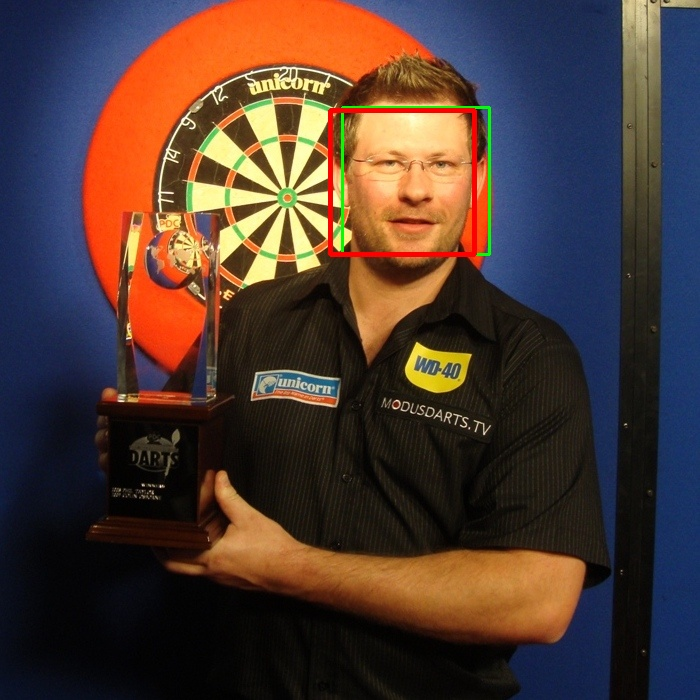
\includegraphics[width=\textwidth, height=20mm, keepaspectratio]{task1/out4.jpg}\label{fig:dart4}}
  \hfill
  \subfloat[dart5.jpg]{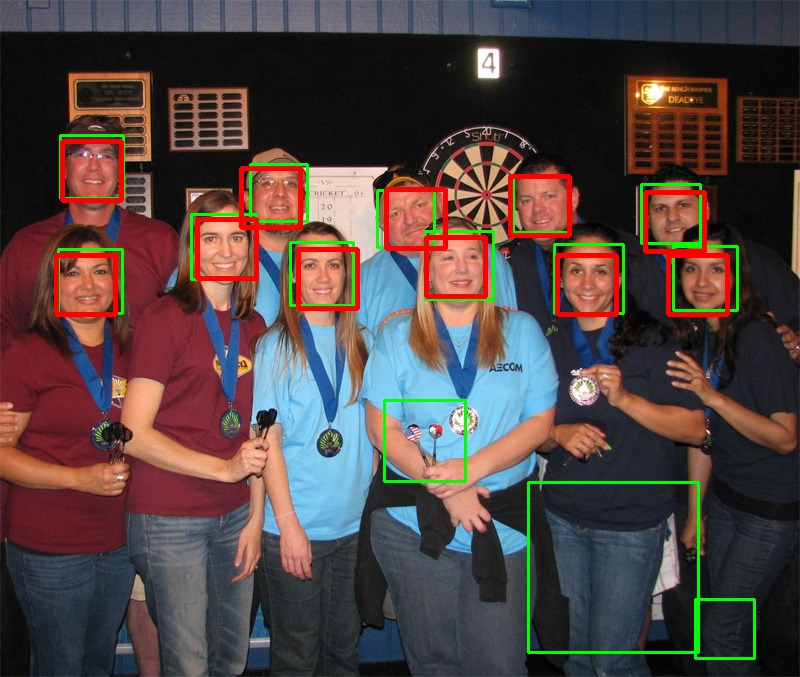
\includegraphics[width=\textwidth, height=20mm, keepaspectratio]{task1/out5.jpg}\label{fig:dart5}}
   \hfill
  \subfloat[dart13.jpg]{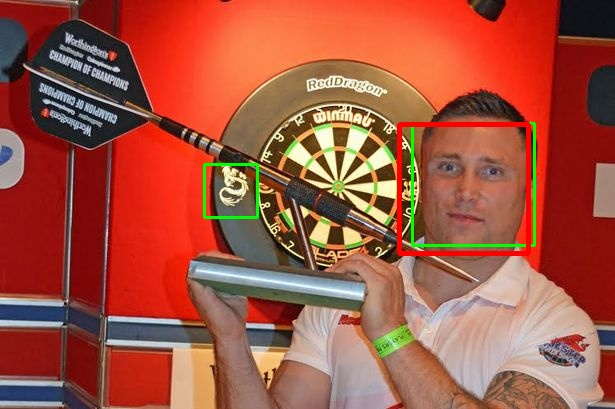
\includegraphics[width=\textwidth, height=20mm, keepaspectratio]{task1/out13.jpg}\label{fig:dart13}}
   \hfill
  \subfloat[dart14.jpg]{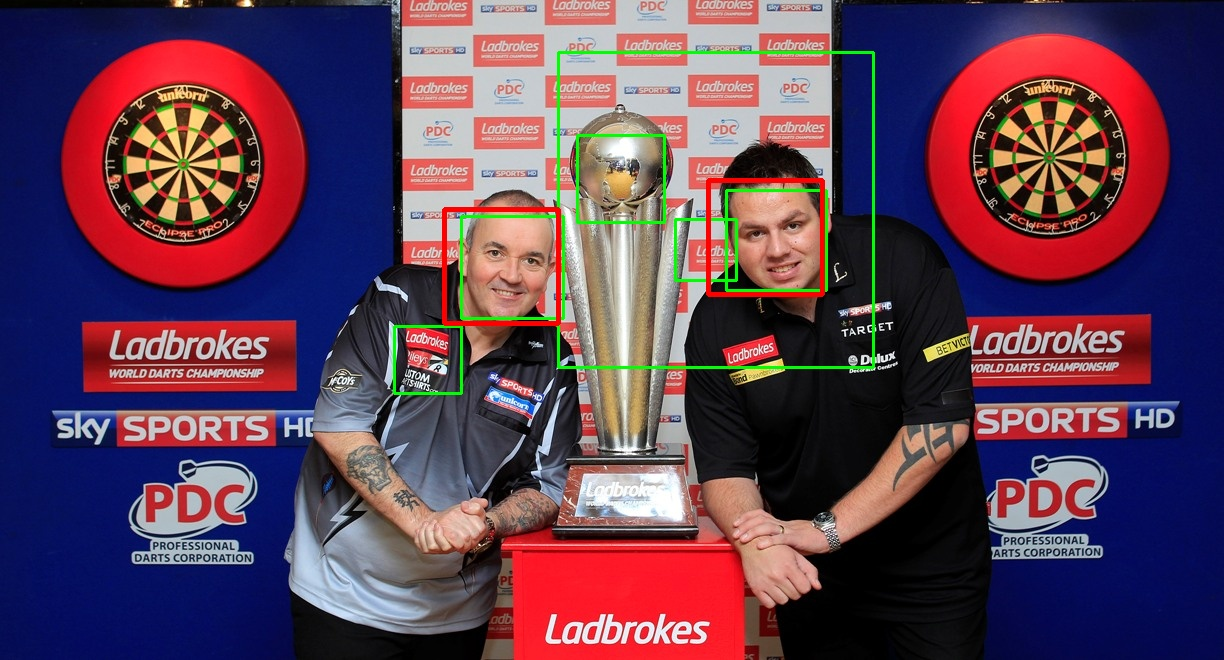
\includegraphics[width=\textwidth, height=20mm, keepaspectratio]{task1/out14.jpg}\label{fig:dart14}}
   \hfill
  \subfloat[dart15.jpg]{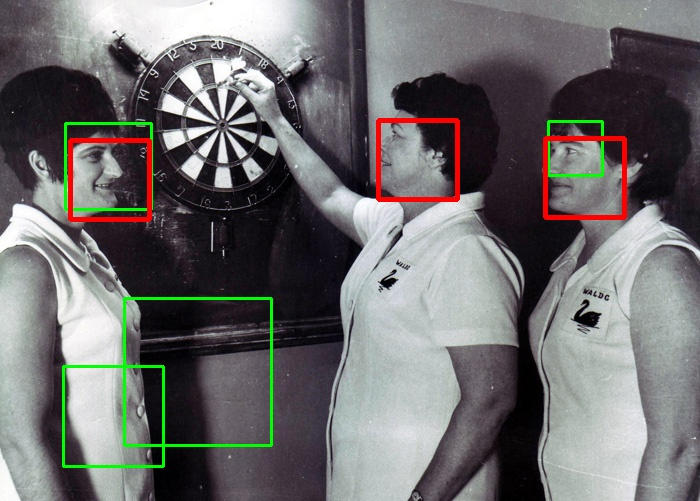
\includegraphics[width=\textwidth, height=20mm, keepaspectratio]{task1/out15.jpg}\label{fig:dart15}}
   \hfill
   \caption{Result of the Viola-Jones Algorithm on human faces (green boxes). Red boxes represent ground truth.}
\end{figure}

\subsection*{Assessing How the Detector Performs}
\vspace{-0.7em}

The TPR or True Positive Rate measures the proportion of relevant items that
are correctly identified. In this case it is the fraction of successfully
detected faces out of all valid faces in an image. The TPR of dart5.jpg and
dart15.jpg are 100\% and 67\% respectfully. A practical difficulty in computing
the TPR accurately is that the ground truth bounding boxes need to be manually
entered in order compare the results of the detector. Also, errors can occur
when faces are side profile as they become ambiguous as to whether they are
valid. It is always possible to get 100\% TRP because one can detect every
possible detection in an image - always resulting in every hit. It will
however, get all the misses too. A better way of evaluating the detector would
be to calculate the \(F_{1}\) score. It takes into account the detectors
precision (PPV - Positive Prediction Value, how many selected items are
relevant) and recall (TPR). A set of rules were created to evaluate whether a
face was valid:


\begin{itemize}
  \item Two eyes and a mouth must be within a boundary to be counted as a hit.
  \item Two eyes and a mouth must be visible to us in order for it to be
    counted as valid.
  \item The \(F_{1}\) score will be calculated by: \[\frac{2 \times P \times
    R}{R + P}\] Where
  \item Recall (TPR) ${P = \frac{true positives}{ground truth}}$.
  \item Precision ${R = \frac{true positives}{true positives + false
    positives}}$.
\end{itemize}

As calculating the F1 score is challenging due to manually counting boxes, a
process was implemented that makes this easier and scalable. It will compare
the centres of the ground truth (which are manually added) and detection boxes.
If the detected bounding box is below a certain threshold, this will be counted
as a true positive. Table 1 below shows the result of this.

\begin{table} [H]
\centering
\begin{tabular}{l| r | r | r | r | r | r}
Picture & Actual & Detected & Hit & Missed & \(F_{1}\) Score \\\hline
dart4 & 1 & 1 & 1 & 0 & 1\\
dart5 & 11 & 14 & 11 & 3 & 0.88 \\
dart13 & 1 & 2 & 1 & 1 & 0.67 \\
dart14 & 2 & 6 & 2 & 4 & 0.5 \\
dart15 & 3 & 4 & 2 & 2 & 0.5
\end{tabular}
\caption{\label{tab:F1}Comparing the \(F_{1}\) Score of different images.}
\end{table}

\section*{Building and Testing the Detector}
\subsection*{Interpreting TPR vs FPR}
\vspace{-0.7em}

Figure 2 shows the training of the detector over the 3 stages. The TPR always
remained as 1, therefore, it was successful in detecting all dartboards. The
decreasing FPR portrays that the detector firstly detects as much as it can,
then reduces the number of objects it detects. As a consequence, it is clear
that the detector is improving. The parameters of the detector were changed to
be optimum. A ratio of 500:1000, positive to negative was used and a maximum
false alarm rate of 0.4.

\begin{figure}[H]
  \centering
  \begin{tikzpicture}
    \begin{axis}[
      title=TPR vs FPR,
      xlabel=$Stage$,
      ylabel=$Rate$
    ]
      \addplot table {task2/TPR.dat};
      \addplot table {task2/FPR.dat};
    \end{axis}
  \end{tikzpicture}
  \caption{TPR (blue) vs FPR (red) across the 3 stages.}
\end{figure}

\subsection*{Testing on images}
\vspace{-0.7em}

\begin{figure}[H]
  \centering
  \subfloat[dart4.jpg.]{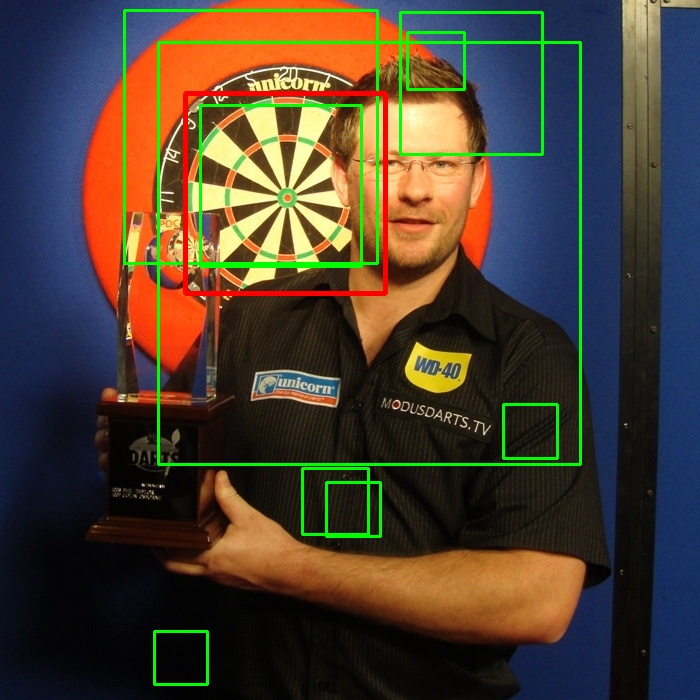
\includegraphics[width=\textwidth, height=20mm, keepaspectratio]{task2/out4.jpg}\label{fig:out4}}
  \hfill
  \subfloat[dart5.jpg]{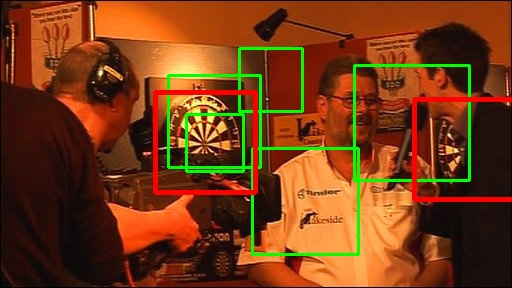
\includegraphics[width=\textwidth, height=20mm, keepaspectratio]{task2/out11.jpg}\label{fig:out11}}
   \hfill
  \subfloat[dart13.jpg]{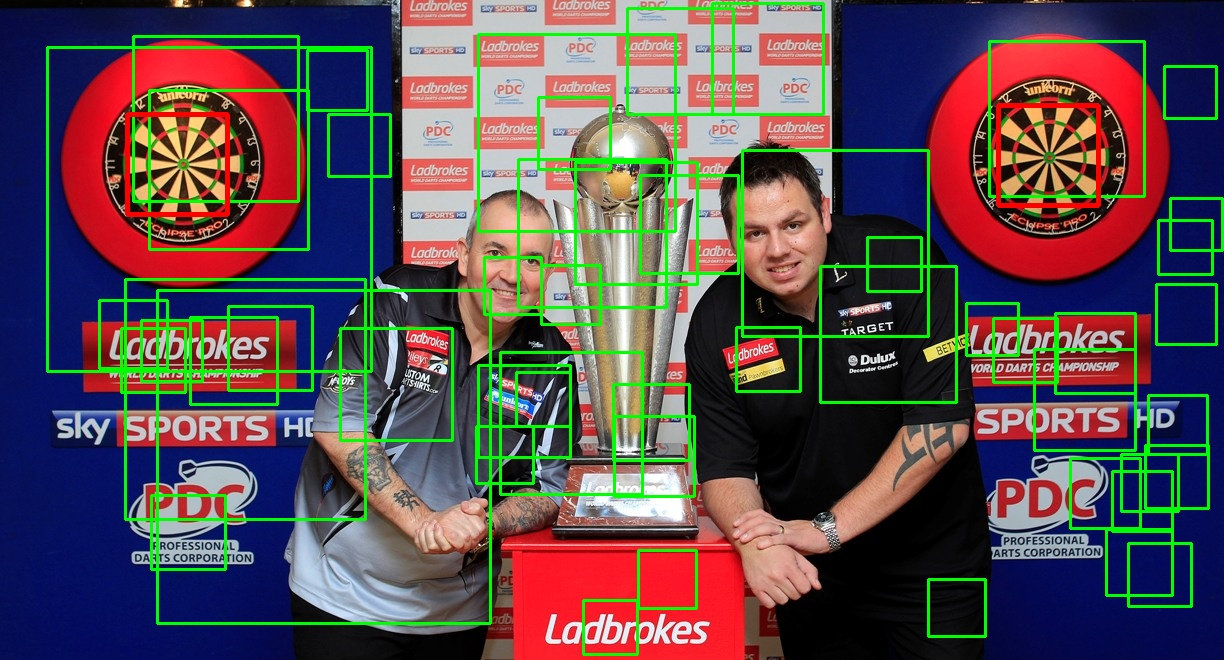
\includegraphics[width=\textwidth, height=20mm, keepaspectratio]{task2/out14.jpg}\label{fig:out14}}
   \hfill
  \subfloat[dart14.jpg]{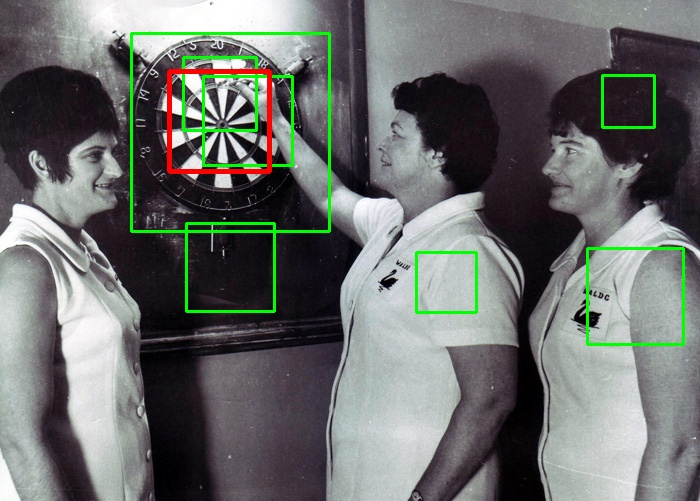
\includegraphics[width=\textwidth, height=20mm, keepaspectratio]{task2/out15.jpg}\label{fig:out15}}
   \hfill
   \caption{Result of the trained dartboard detector.}
\end{figure}

The \(F_{1}\) of the images are:
\begin{multicols}{4}
    \begin{itemize}
		\item dart0.jpg - 0.14.
        \item dart1.jpg - 0.13.
        \item dart2.jpg - 0.12.
        \item dart3.jpg - 0.20.
        \item dart4.jpg - 0.20.
        \item dart5.jpg - 0.10.
        \item dart6.jpg - 0.17.
        \item dart7.jpg - 0.09.
        \item dart8.jpg - 0.13.
        \item dart9.jpg - 0.13.
        \item dart10.jpg - 0.11.
        \item dart11.jpg - 0.29.
        \item dart12.jpg - 0.33.
        \item dart13.jpg - 0.14.
        \item dart14.jpg - 0.07.
        \item dart15.jpg - 0.25.
    \end{itemize}
\end{multicols}

The overall \(F_{1}\) score is consequently 0.1625. The \(F_{1}\) score is
relatively low meaning the denominator is much bigger concluding that there was
a high number of detections with respect to hits. This means that there were a
lot of false positives. The usefulness of the plot (Figure 2) is that it can be
clearly seen that the detector is currently under fitting - the TPR remains at
1 while the FPR decreases. This fact, along with the \(F_{1}\) scores, portray
the results of a poor detector. However, it can be used to an advantage. The
under fitting can be combined with other classifying detectors in order to
improve results.
\\\\

\section*{Integration with Shape Detectors}
\subsection*{Image Results}
Below are some resulting images from our improved detector.


\vspace{-2em}
\begin{figure}[H]
  \centering
  \subfloat[Threshold Gradient Magnitude.]{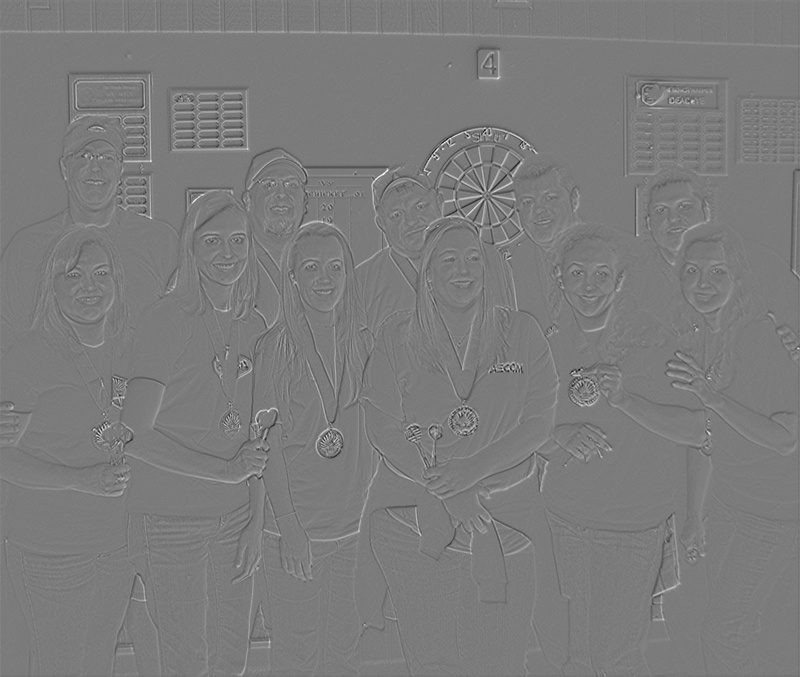
\includegraphics[width=\textwidth, height=20mm, keepaspectratio]{task3/mag5.jpg}\label{fig:mag1}}
  \hfill
  \subfloat[Hough Space]{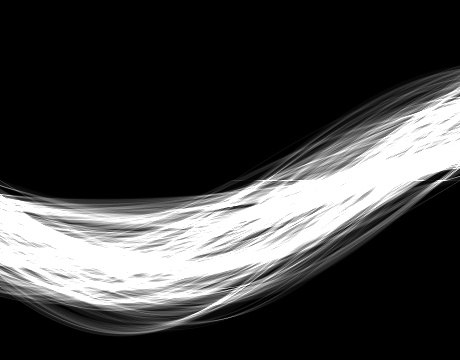
\includegraphics[width=\textwidth, height=20mm, keepaspectratio]{task3/hough5.jpg}\label{fig:hough1}}
   \hfill
  \subfloat[Result]{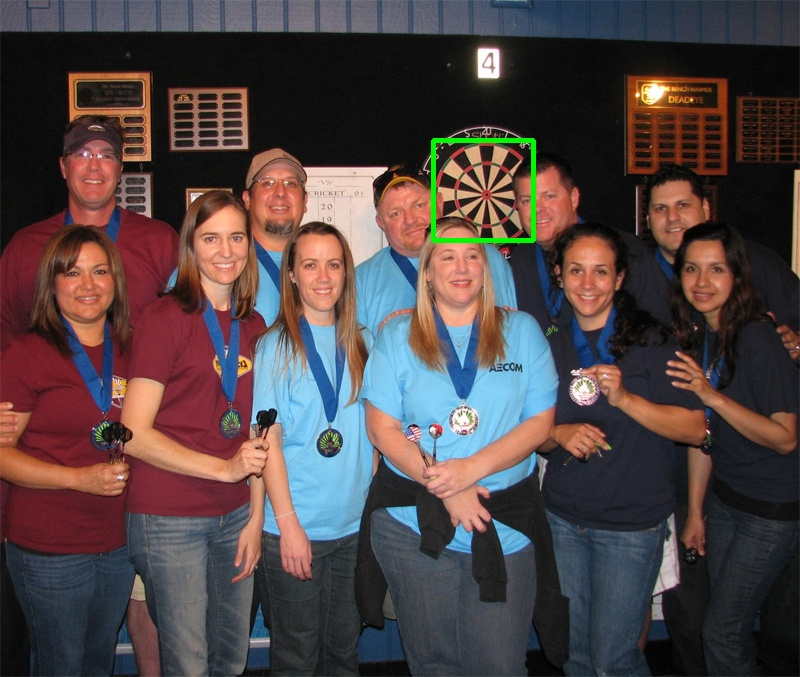
\includegraphics[width=\textwidth, height=20mm, keepaspectratio]{task3/out5.jpg}\label{fig:result1}}
   \hfill
   \caption{dart5.jpg shows the merits of the detector.}
\end{figure}
\vspace{-2.5em}

\begin{figure}[H]
  \centering
  \subfloat[Threshold Gradient Magnitude.]{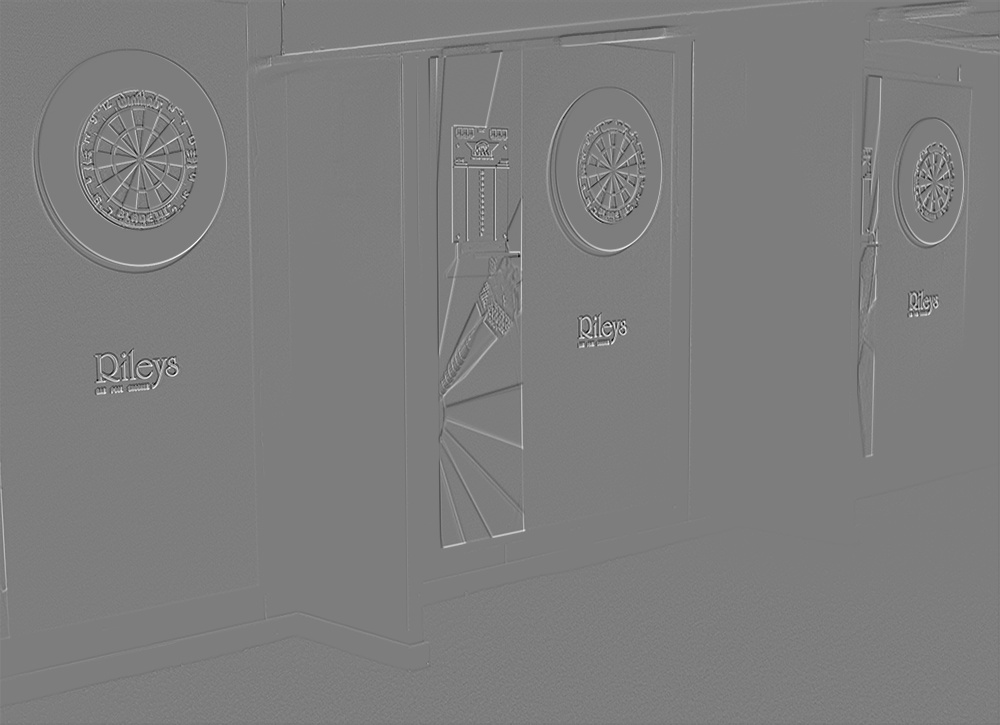
\includegraphics[width=\textwidth, height=20mm, keepaspectratio]{task3/mag10.jpg}\label{fig:mag2}}
  \hfill
  \subfloat[Hough Space]{
\includegraphics[width=\textwidth, height=20mm, keepaspectratio]{task3/hough10.jpg}\label{fig:hough2}}
   \hfill
  \subfloat[Result]{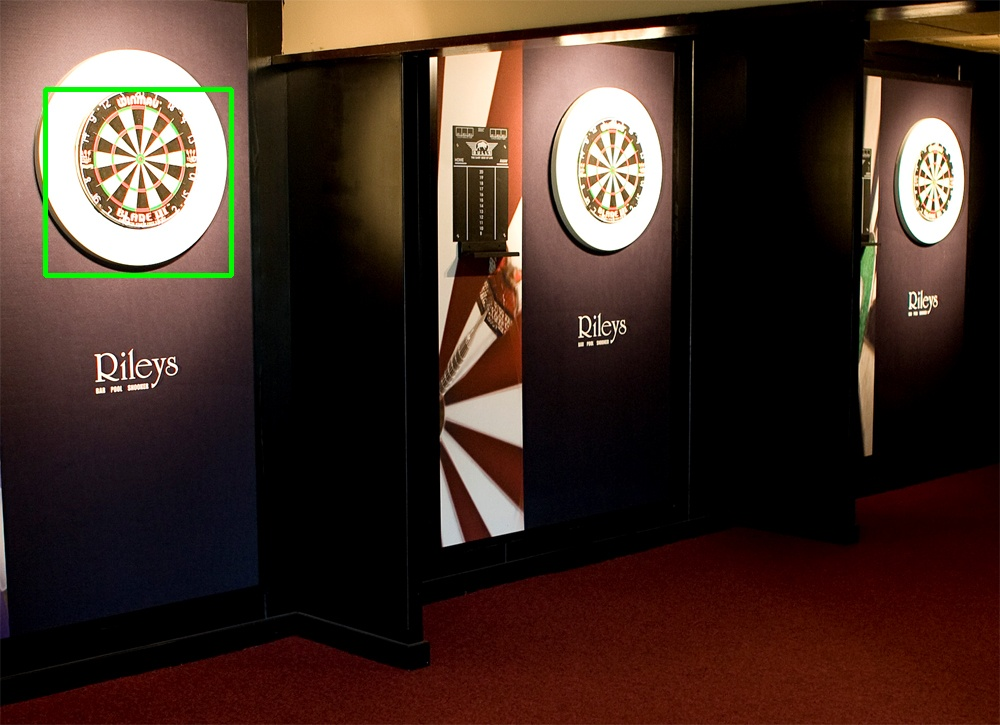
\includegraphics[width=\textwidth, height=20mm, keepaspectratio]{task3/out10.jpg}\label{fig:result2}}
   \hfill
   \caption{dart10.jpg shows the limitations of the detector.}
\end{figure}

The new dartboard detector did considerably better than the previous, achieving
an overall \(F_{1}\) score 0.767 with the previous being 0.163.

\subsection*{Merits and Limitations}
\vspace{-0.7em}
\begin{itemize}
    \item This detector adds more classifiers when analysing images meaning
      that the large set of detections with many negative hits can be reduced
      by combining each classifier result. This detector works optimally with
      images where dartboards are in good lighting and are facing straight at
    the camera in the scene.
  \item As shown in the \textit{dart10.jpg} image, the detector will fail to
    detect dartboards that are at an angle. These failures are due to the
    circle and line Hough transformation being used that struggle to detect
    such non-uniform shapes.
    \item Our overall average precision became 0.767 with a true positive rate
      of 0.833 resulting in correctly detecting 16 out of a possible 21
      dartboards with 5 false positives.
\end{itemize}

\subsection*{Combination of Detectors}
\begin{figure}[H]
  \centering
  \subfloat[Flowchart representing the detector.]{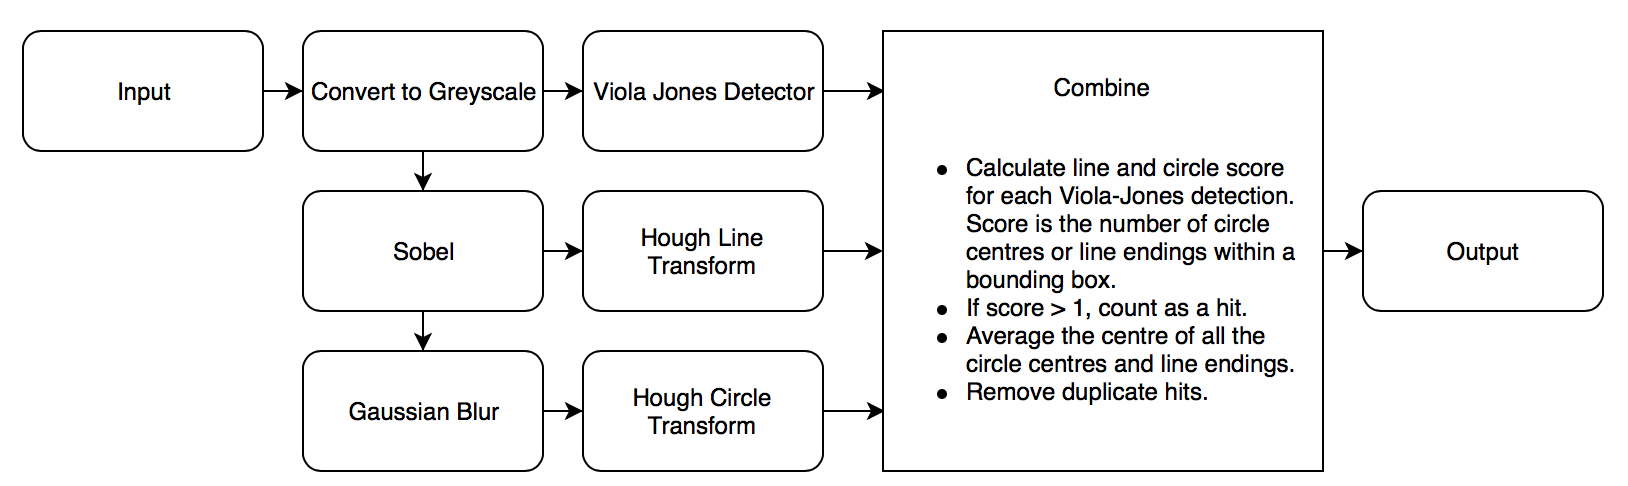
\includegraphics[width=\textwidth, height=40mm, keepaspectratio]{task3/flowchart.png}\label{fig:flowchart}}
\end{figure}

\begin{itemize}
    \item Our approach was to create new classifiers which would refine the
      large set of negative and positive hits of the Viola Jones detector down
      to only true positives by accepting Viola Jones hits that were also
      observed by the line and circle detectors.
    \item Line detections are achieved by accepting a hit when a large number
      of lines intersect at a pixel position, relative to the number of lines
      found in the image via the Hough transformation. This involves iterating
      through the set of Viola hits, comparing whether any line or circle hits
      are contained in the Viola bounding box, accepting if so, rejecting
      otherwise. Accepted hits would change its location based on the average position of itself, along with its combined detections.
    \item Circle detections also give the ability to estimate the size of the
      dartboard. Furthermore, it takes the average radii of included circles
      and includes this in the approximation.
    \item To reduce duplicate detections of the same dartboard, overlapping
      bounding boxes are combined, also averaging location and size - ensuring
      one positive hit per dartboard.
\end{itemize}



\section*{Improving the Detector}

\begin{itemize}
\item In order to improve our dartboard classifier, we considered further
  shapes which help to classify a dartboard being present.  As such, we
    identified two shapes - ellipses and triangles. Firstly, we realised that
    some dartboards had been not been identified by our classifier due to not
    being detected by circles with dartboards that are at an angle. By using
    ellipses, we would be able to capture this shape of valid dartboards. We
    also chose to consider triangles as all dartboards have distinct triangles
    contained that will give more detections to be combined.

\item Detecting both triangle and ellipse shapes is achieved by first applying
  the Canny edge detector on the grey scale input image. The Canny edge
    detector [1] works by calculating the gradient magnitude of each pixel. To
    determine whether each pixel is part of an edge, two thresholds are applied
    where pixels greater than the high threshold are considered pixels on an
    edge, pixels below the low threshold are discarded and pixels in-between
    the two thresholds are considered edges only if they are connected to a
    pixel that is above the higher threshold.  In order to select an
    appropriate threshold for each image, the Otsu method is applied.  [2]

\item The Otsu method is used to determine the largest threshold input for the
  Canny edge detector. It assumes that the image contains two classes of
    pixels. It then calculates the optimum threshold and partitions the two
    classes so that their combined variance is maximal. We selected our minimal
    threshold to be one third of the maximum gradient the Otsu method returned.

\item With our Canny image we then used the \textit{findCountours} function
  which attempts to find groups of points which together form a curve. With
    these contours we can then determine whether, in the case of triangles,
    they form a closed shape of 3 sides, or in the case of ellipses, a contour
    group with many elements is indicative of a many sided shape - an ellipse.

\item In combination with the new shapes being in included into our detector,
  we also investigated another type of image processing technique called
    \textit{Speeded Up Robust Features} (SURF) - a speeded up version of
    \textit{Scale-invariant feature transform} (SIFT) [3]. This method aims to
    take feature vectors of some image, the input object, which are independent
    of scaling, translation and rotation. Using the opencv SURF detector, we
    evaluated keypoint features of the dartboard image \textit{dartboard.jpg}.
    These keypoints are then aimed to be matched against the keypoints of our
    test images with dartboard in. The resulting matches can then be used as
    another set of detection data when combining.

\item With the matched keypoint values found on out test images using SURF, we
  cluster all neighbouring points as these should be of the same object, and
    then combine them into our Viola Jones detections like before. Detected
    triangles and ellipses are also combined.


\end{itemize}
Including these approaches into our detector, out new \(F_{1}\) score has imrpoved to 0.838.


\vspace{-2em}
\begin{figure}[H]
  \centering
  \subfloat[dart10.jpg Overlay Detections]{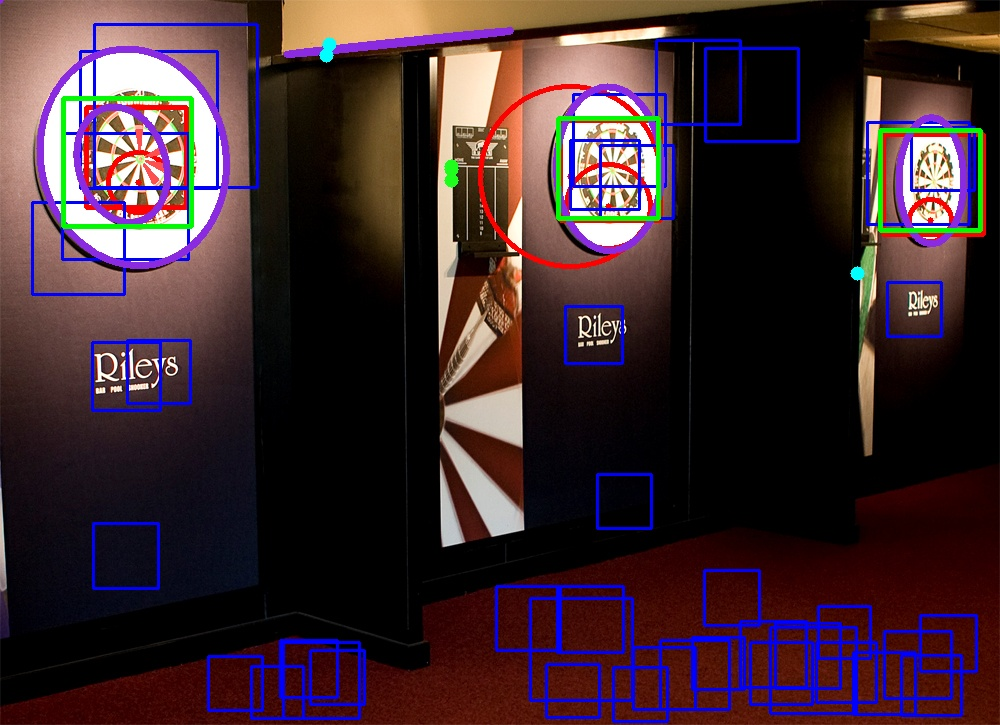
\includegraphics[width=\textwidth, height=20mm, keepaspectratio]{task4/overlay/out10.jpg}\label{fig:result4}}\hfill
  \subfloat[dart10.jpg Result]{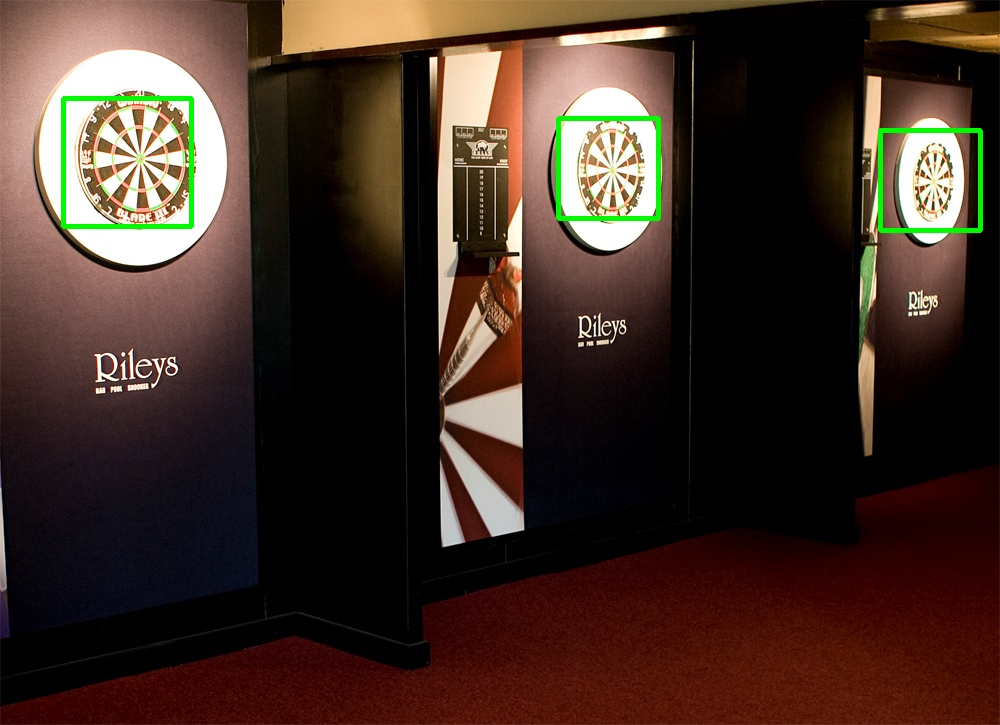
\includegraphics[width=\textwidth, height=20mm, keepaspectratio]{task4/alldecs/out10.jpg}\label{fig:result4}}\hfill
  \subfloat[dart11.jpg Overlay Detections]{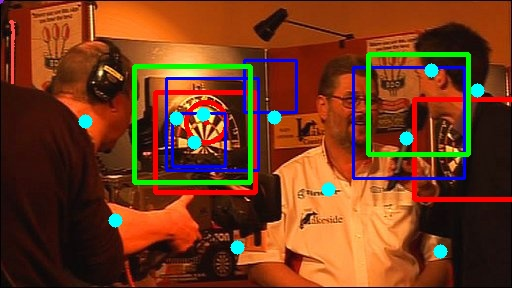
\includegraphics[width=\textwidth, height=20mm, keepaspectratio]{task4/overlay/out11.jpg}\label{fig:result4}}\hfill
  \subfloat[dart11.jpg Results]{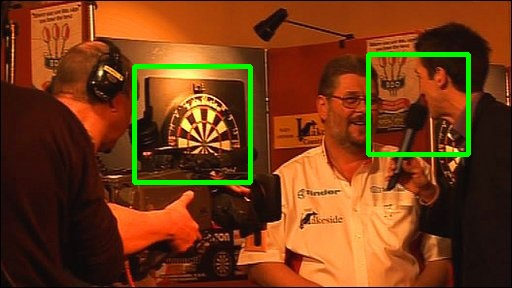
\includegraphics[width=\textwidth, height=20mm, keepaspectratio]{task4/alldecs/out11.jpg}\label{fig:result4}}\hfill
\end{figure}

\subsection*{Merits and Limitations}
Including our new detection techniques, we are now able to detect dartbaords
that are at an angle as well as obscured from view, which we previously could
not. Although our detector now performs better than before, we have also
introduced more false positives into our results. This is due to the fact that
as we include more data from new classifiers, we also increase the data set
that represent false positives, increasing the chance of falsely detecting.


\section*{References}

\begin{enumerate}
\item http://citeseerx.ist.psu.edu/viewdoc/download?doi=10.1.1.420.3300\&rep=rep1\&type=pdf
\item https://en.wikipedia.org/wiki/Otsu\%27s\_method
\item http://opencv-python-tutroals.readthedocs.io/en/latest/py\_tutorials/py\_feature2d/py\_surf\_intro/py\_surf\_intro.html
\end{enumerate}

\vspace{-4em}
\end{document}
